\section{Video Input}
This section describes the effort that was put into getting camera input for the system (functional requirement FR3).
Throughout the working period the approach to this was changed multiple times as we learned more about the hardware we were working with.

\subsection{Raspberry Pi Camera}
After some consideration it was decided that the \textit{Raspberry Pi Camera Board}\footnote{\url{https://www.raspberrypi.org/products/camera-module/}} (PiCamera) would be used as the camera module for the system.
The circumstances leading to this choice are discussed in Section \ref{sec:camera_discussion}.

\begin{figure}[h]
    \centering
    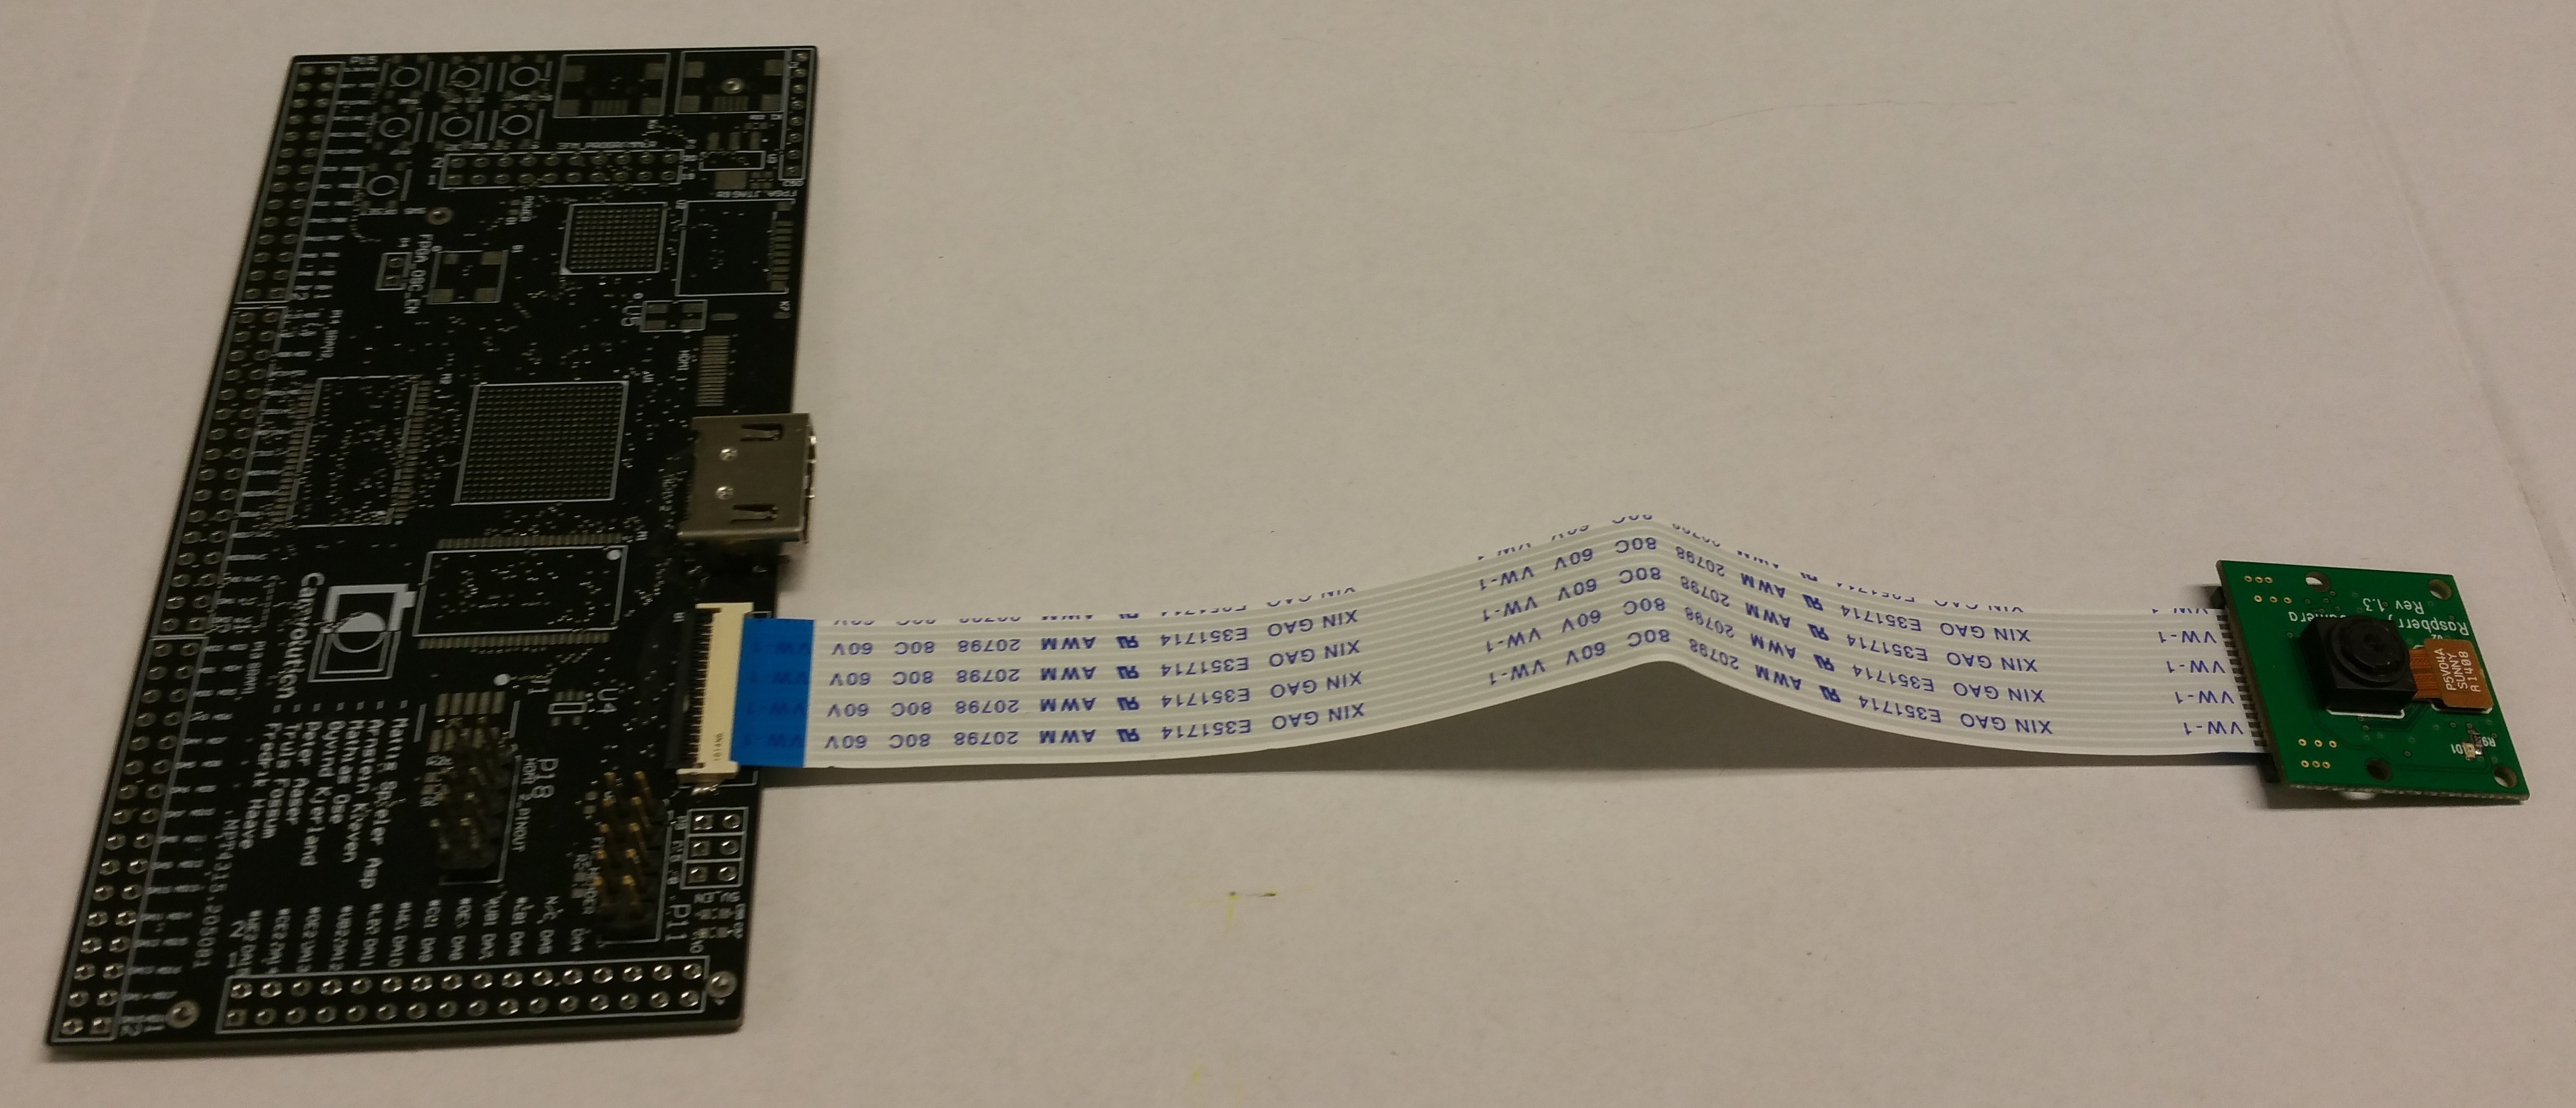
\includegraphics[width=0.75\textwidth]{img/picamera}
    \caption{Raspberry Pi Camera connected to Camvolution board}
\end{figure}

The \textit{Raspberry Pi Foundation} has designed this peripheral for use with the \textit{Raspberry Pi} computer.
The PiCamera can take still shots as well as record continuous video.
The module consists of a camera sensor on a board with a controller unit which connects to the Pi (or another master device) via a 16-pin ribbon cable.
Communication over this cable is defined by the proprietary \textit{MIPI Camera Serial Interface} (CSI) specification.

The master device controls the camera module by sending instructions over an I2C bus on the ribbon cable,
and the camera module responds with picture data over two clocked differential busses.\cite{picam-pinout}
Parameters that may be controlled include video encoding, resolution in two dimensions and framerate.


\subsection{SD Card Video}
One possible source of video is a file stored on the SD card connected to the board.
The MCU is able to open files and pass the data from it to the processor over EBI.
For simplicity of development the MCU should not need to handle encoded video. Instead, the video files should contain raw pixel data so that it can easily be streamed to the processor.


\subsection{Options for Video Path}
\begin{figure}
    \centering
    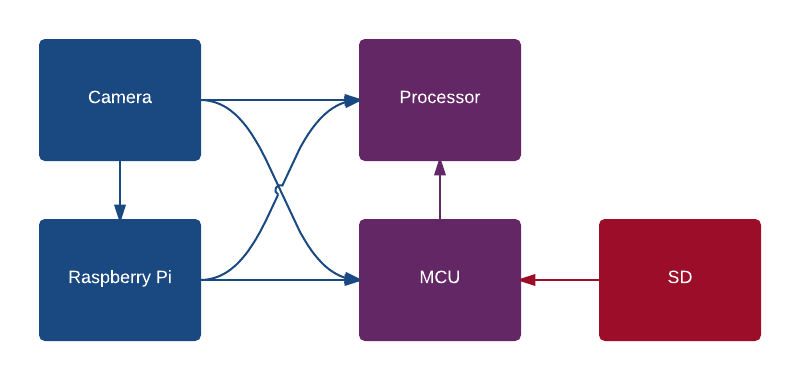
\includegraphics[width=\linewidth]{img/VideoPath}
    \caption{Paths an input video stream could take to reach the processor.}
    \label{fig:VideoPath}
\end{figure}

Because the group had no experience with video input,
there was a lot of uncertainty of how to transfer video from the camera to the processor.
What we decided we wanted to do was to have both video camera and data from SD card as possible sources,
with the possibility to switch between them by using the buttons on the board.
Figure \ref{fig:VideoPath} shows an overview of the possible paths a video stream could take from the camera,
and some options that were explored are briefly outlined below:

\begin{description}
    \item[PiCamera Connected to the Board, Controlled by the MCU]
        \hfill\\
        Wiring the camera connector to the MCU, having software on the MCU control the camera and receive the video stream before forwarding it to the FPGA.
    \item[PiCamera Connected to the Board, Controlled by the FPGA]
        \hfill\\
        Wiring the camera connector directly to the FPGA, having an FPGA submodule control the camera and receive the video stream.
    \item[PiCamera Connected to a Raspberry Pi, Transfer Over With Bus]
        \hfill\\
        Having the Raspberry Pi control the camera using the provided libraries.
        Transfer video stream to Camvolution using a parallel bus controlled by GPIO software.
    \item[PiCamera Connected to a Raspberry Pi, Transfer With SPI]
        \hfill\\
        Having the Raspberry Pi control the camera using the provided libraries.
        Transfer the video stream to Camvolution using built-in SPI hardware.
    \item[SD Card Video]
        \hfill\\
        Instead of using the camera, have a recorded video stored on the SD card which the MCU can forward to the FPGA.
    \item[HDMI Input]
        \hfill\\
        Instead of using the camera, use the second HDMI port on the board for input from any HDMI source.
\end{description}

\subsection{Reverse-Engineering the Camera Control Protocol}
\begin{figure}
    \centering
    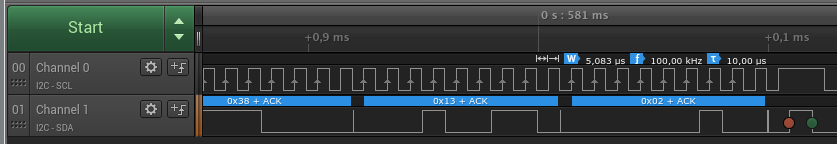
\includegraphics[width=\linewidth]{img/logic/pi_cam_i2c}
    \caption{I2C communication between Raspbery Pi and PiCamera}
    \label{fig:PiCamI2C}
\end{figure}

The Raspberry Pi controls the PiCamera by sending signals over a two-wire serial bus (I2C).
In order to make use of the PiCamera, it is necessary to reimplement the control system.
Since there is little documentation online, this must be reverse-engineered.
An attempt was made to use a logic analyzer to "listen in" on the communication between the Raspberry Pi and PiCamera.
A screenshot of this can be seen in Figure \ref{fig:PiCamI2C}.

